% https://tex.stackexchange.com/a/52703/173708

% (S) -> (M) -> (V) -> (shuffle) -> (P) -> (R) - (F)
% S for Start F for Final
\documentclass{standalone}
\usepackage{tikz}
\usetikzlibrary{%
  calc,
  fit,
  shapes,
  backgrounds
}
% the next macro is useful to create a table
\newcommand\tabins[3]{%
 \tikz[baseline=(Tab.base)] 
           \node  [rectangle split, 
                   rectangle split parts=3, 
                   draw, 
                   align=right,
                   inner sep=.5em,
                   rectangle split horizontal] (Tab)
                           {\hbox to 4ex{#1}
           \nodepart{two}  {\hbox to 8ex{\hfill #2\$}}  
           \nodepart{three}{\hbox to 3ex{#3}}}; 
}

\begin{document}
\parindent=0pt
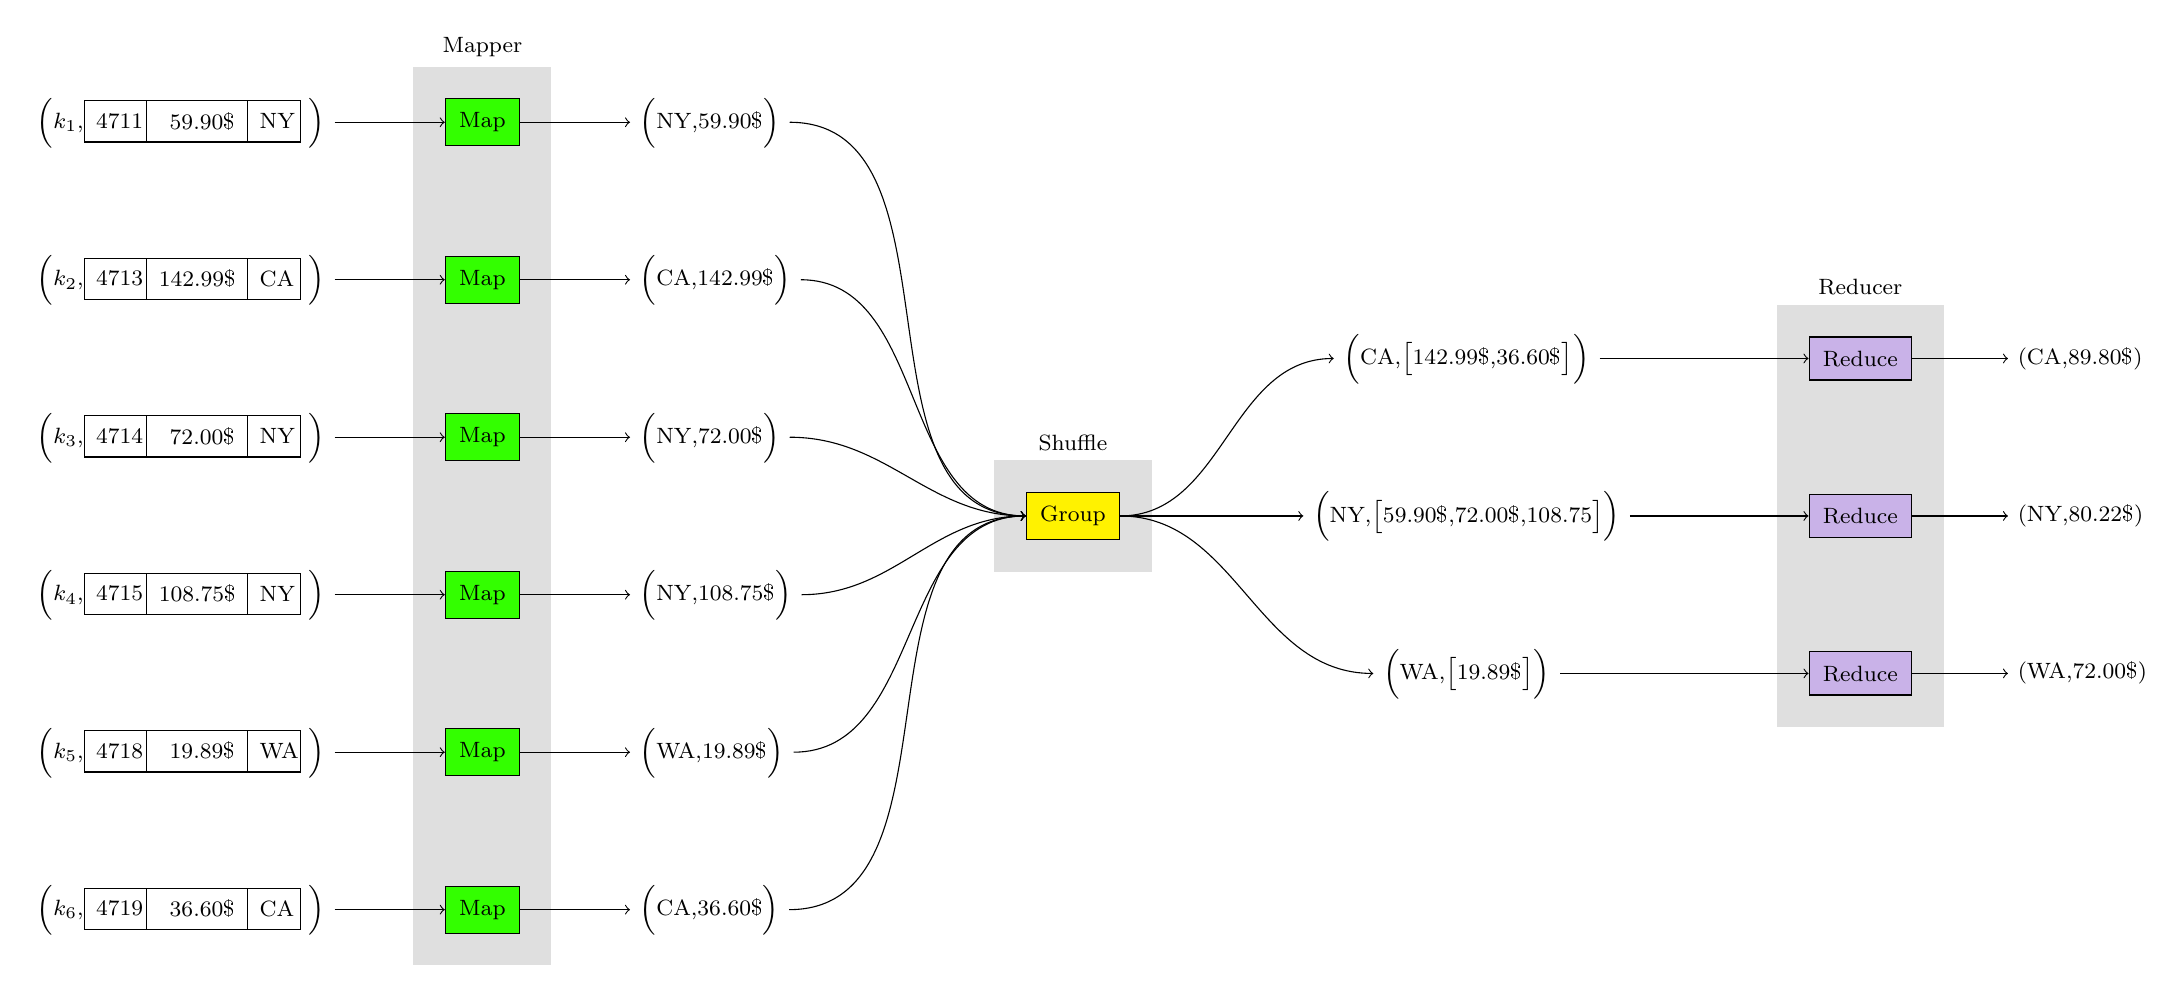
\begin{tikzpicture}[%
   %every node/.style={transform shape},% now it's not necessary but good for a poster
  x=1.25cm,y=2cm,  
  font=\footnotesize,
  % every group of nodes have a style except for main, the style is named by a letter
  main/.style={draw,fill=yellow,inner sep=.5em},
  R/.style={draw,fill=purple!40!blue!30,inner sep=.5em},
  M/.style={draw,fill=green!80!yellow,inner sep=.5em},
  S/.style={anchor=east},
  V/.style={anchor=west},
  P/.style={anchor=center},
  F/.style={anchor=west}
  ]

% main node the reference Shuffle 
\node[main] (shuffle) {Group};
%group R reducer
\node[R] at ($(shuffle)+(8,1)$)    (R1+) {Reduce};
\node[R] at ($(shuffle)+(8, 0)$)   (R0)  {Reduce};
\node[R] at ($(shuffle)+(8,-1)$)   (R1-) {Reduce};
% group M Mapper
\node[M] at ($(shuffle)+(-6,+2.5)$)   (M3+)  {Map};
\node[M] at ($(shuffle)+(-6,+ 1.5)$)  (M2+)  {Map};
\node[M] at ($(shuffle)+(-6,+ .5)$)   (M1+)  {Map};
\node[M] at ($(shuffle)+(-6,- .5)$)   (M1-)  {Map};
\node[M] at ($(shuffle)+(-6,- 1.5)$)  (M2-)  {Map};
\node[M] at ($(shuffle)+(-6,-2.5)$)   (M3-)  {Map};
% group S Start the first nodes
\node[S] at ($(M3+)+(-1.5,0)$)  (S3+) {\Big($k_1$,\tabins{4711}{59.90}{NY}\Big)};
\node[S] at ($(M2+)+(-1.5,0)$)  (S2+) {\Big($k_2$,\tabins{4713}{142.99}{CA}\Big)};
\node[S] at ($(M1+)+(-1.5,0)$)  (S1+) {\Big($k_3$,\tabins{4714}{72.00}{NY}\Big)}; 
\node[S] at ($(M1-)+(-1.5,0)$)  (S1-) {\Big($k_4$,\tabins{4715}{108.75}{NY}\Big)}; 
\node[S] at ($(M2-)+(-1.5,0)$)  (S2-) {\Big($k_5$,\tabins{4718}{19.89}{WA}\Big)};  
\node[S] at ($(M3-)+(-1.5,0)$)  (S3-) {\Big($k_6$,\tabins{4719}{36.60}{CA}\Big)};  
% group V  why not
\node[V] at ($(M3+)+(1.5,0)$)  (V3+) {\Big(NY,59.90\$\Big)};
\node[V] at ($(M2+)+(1.5,0)$)  (V2+) {\Big(CA,142.99\$\Big)};
\node[V] at ($(M1+)+(1.5,0)$)  (V1+) {\Big(NY,72.00\$\Big)}; 
\node[V] at ($(M1-)+(1.5,0)$)  (V1-) {\Big(NY,108.75\$\Big)}; 
\node[V] at ($(M2-)+(1.5,0)$)  (V2-) {\Big(WA,19.89\$\Big)};  
\node[V] at ($(M3-)+(1.5,0)$)  (V3-) {\Big(CA,36.60\$\Big)};   

\node[P] at ($(R1+)+(-4,0)$) (P1+) {\Big(CA,\big[142.99\$,36.60\$\big]\Big)};
\node[P] at ($(R0) +(-4,0)$) (P0)  {\Big(NY,\big[59.90\$,72.00\$,108.75\big]\Big)};
\node[P] at ($(R1-)+(-4,0)$) (P1-) {\Big(WA,\big[19.89\$\big]\Big)}; 

\node[F] (F1+) at ($(R1+)+(1.5,0)$) {(CA,89.80\$)};
\node[F] (F0)  at ($(R0) +(1.5,0)$) {(NY,80.22\$)}; 
\node[F] (F1-) at ($(R1-)+(1.5,0)$) {(WA,72.00\$)}; 

% wrappers
\begin{scope}[on background layer]
    \node[fill=lightgray!50,inner sep = 4mm,fit=(shuffle),label=above:Shuffle] {}; 
\end{scope} 
\begin{scope}[on background layer]
    \node[fill=lightgray!50,inner sep = 4mm,fit=(R1+)(R1-),label=above:Reducer] {}; 
\end{scope}  
\begin{scope}[on background layer]
    \node[fill=lightgray!50,inner sep = 4mm,fit=(M3+)(M3-),label=above:Mapper] {}; 
\end{scope}

%edges

\foreach \indice in {3+,2+,1+,1-,2-,3-} \draw[->] (S\indice.east) -- (M\indice.west); 
\foreach \indice in {3+,2+,1+,1-,2-,3-} \draw[->] (M\indice.east) -- (V\indice.west);
\foreach \indice in {3+,2+,1+,1-,2-,3-} \draw[->] (V\indice.east) to [out=0,in=180] (shuffle.west); 
\foreach \indice in {1+,0,1-} \draw[->] (shuffle.east) to [out=0,in=180] (P\indice.west);  
\foreach \indice in {1+,0,1-} \draw[->] (P\indice.east) -- (R\indice.west);
\foreach \indice in {1+,0,1-} \draw[->] (R\indice.east) -- (F\indice.west);   
\end{tikzpicture} 

\end{document}     